\chapter{Literature study}
\label{chap:literature}

This chapter presents an overview of literature that is related to this work. The first section will summarize the mobile application architectures that are currently used to create cross-platform solutions. In the second section, a generic software evaluation and selection methodology will be explored. In the third and last section, a number of techniques for multi-criteria decision making are studied, together with their strengths and weaknesses.

\section{Mobile application architectures}

Building cross-platform solutions starts at the architectural level. This section will discuss the architectures that are currently used with mobile applications or apps for short \cite{Friese}. Mobile architectures comprise of three key elements: 

\begin{itemize}
    \item The \emph{mobile device} is the piece of hardware that runs the actual application. This is the place where the architectures will differ the most.
    \item The \emph{backend} is a service, provided by one or more servers that store all the application data. This could be a web service, ERP software like SAP, a CRM system like Salesforce, etc. or it could be a combination of such services.
    \item The \emph{mobile hub} or\emph{mobile orchestrator} is a server that acts as a mediator between the mobile device and the backend. It is put in place for multiple reasons: it exposes a uniform interface to the mobile device (and hides external API changes), prevents distributed denial-of-service (DDoS) attacks from the large number of mobile devices connecting to the backend, can cache information to reduce the load on the backend, can inject services like advertising into the application, etc.
\end{itemize}

The architecture of the native application is discussed first and is used as a reference architecture. For each of these architecture, a number of aspects will be highlighted: performance, look \& feel, platform access, programming languages, development cost and distribution.

\subsection{Native application}

A native application is an application that is specifically designed to run on a particular platform. It is the default approach to develop applications for mobile devices and is therefore considered the reference architecture in this section. It is illustrated in \fref{fig:native}. 

\begin{figure}[h]
    \begin{center}
        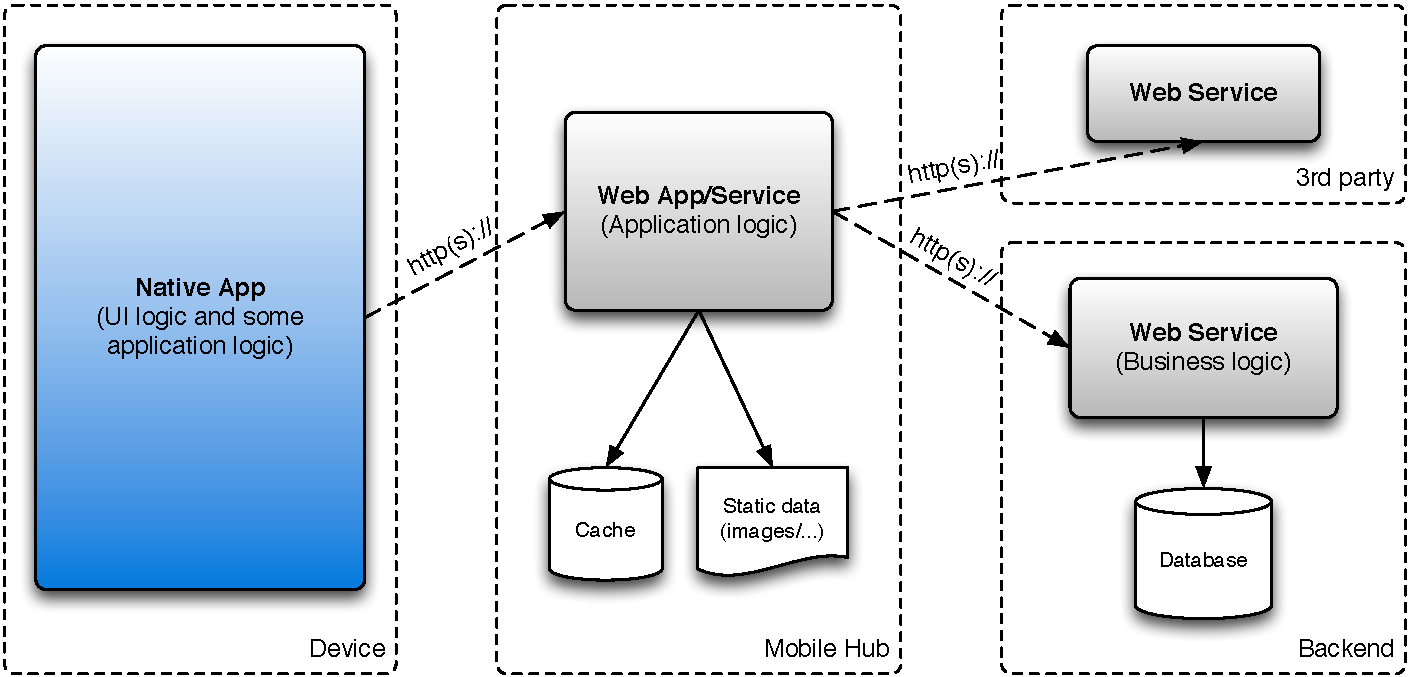
\includegraphics[width=\textwidth]{figs/native.pdf}
        \caption{Architecture of a native application. Based on \cite{Friese}}
        \label{fig:native}
    \end{center}
\end{figure}

Native applications are developed with the supplied software development kit (SDK). That SDK uses a particular programming language that developers will have to learn together with the features of the SDK. In return they will get full access to the platform and its features. As a result, the best performance can be achieved with this kind of application.

The SDK also provides a large number of user interface elements that developers can use to create a rich user interface that is consistent with the look \& feel of the platform. This is called native look \& feel. Native apps are typically distributed through an online marketplace like the App Store for iOS applications or Google Play for Android applications. 

The development cost of native applications is high because developers need to be familiar with multiple SDKs and the application has to be developed separately for every platform that has to be supported.

\subsection{Mobile web application}

Mobile web applications are websites that are optimized for mobile browsers. Since every platform comes with a browser, this is the easiest way to get an application running on all platforms. An overview of this architecture is depicted in \fref{fig:web}. Mobile web applications are built with HTML (content), JavaScript (behaviour) and CSS (styling, are viewed in the browser and are distributed on the Internet with a URL but they cannot be installed on the device. A workarounds using Web Clips \cite{Safari:webclips} is available on iOS and on Android, bookmarks can be placed on the home screen. 

\begin{figure}[h]
    \begin{center}
        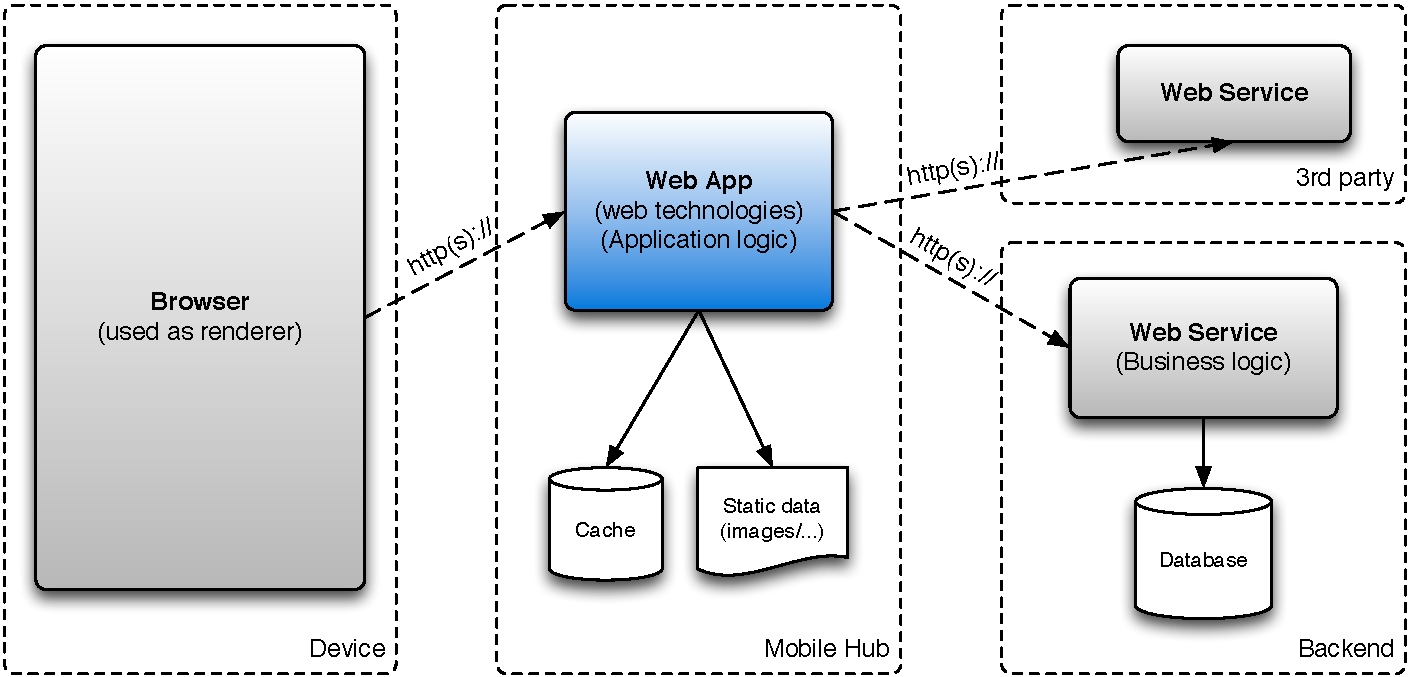
\includegraphics[width=\textwidth]{figs/web.pdf}
        \caption{Architecture of a mobile web application. Based on \cite{Friese}}
        \label{fig:web}
    \end{center}
\end{figure}

Mobile web applications are not nearly as powerful as native applications because the web is currently not a first-class platform. Many mobile web browsers lack support for particular HTML5 features. These defects are listed on websites like ``Can I use...''\footnote{\url{http://caniuse.com}} and ``Mobile HTML5''\footnote{\url{http://mobilehtml5.org}}. Developers should constantly check whether a certain feature is available. In some cases, the missing feature can be \emph{polyfilled}. This term polyfill is inspired by the famous wall filler ``Polyfilla'' and is used for additional pieces of code that provide the missing HTML5 functionality. However, no polyfill can provide access to the underpinning hardware. Most mobile web applications also require an internet connection because the application is not cached in the browser. 

Mobile web applications cannot make use of the native user interface elements. Because of this limitation, it is hard to provide a native look \& feel. There are a number of project that try to mimic the native user interface elements with HTML templates and custom styles. However, the styling is quite complex and additional behaviour is added to animate these elements, which is disadvantageous for the performance. On the other hand, some people believe that the web is a platform of its own because it satisfies the ``one size that fits all'' philosophy. Therefore, it is entitled to its own look \& feel \cite{Mahemoff:2011}.

The development cost of mobile web applications is low because it does not require additional skills (web development is often already in the skill portfolio) and the application has to be developed only once and can serve all platforms. 

\subsection{Hybrid application}

A Hybrid application is the combination of a native application and a mobile web application. The actual application is a mobile web application that is embedded in a native application and made visible through a WebView\footnote{A WebView is a native user interface element that displays web content inside applications.}. The native shell offers a JavaScript bridge to the web application, allowing the web application to access to the system. Because hybrid applications and wrapped in a native shell, they can be distributed through (official) marketplaces. The architecture is visualized in \fref{fig:hybrid}.

\begin{figure}[h]
    \begin{center}
        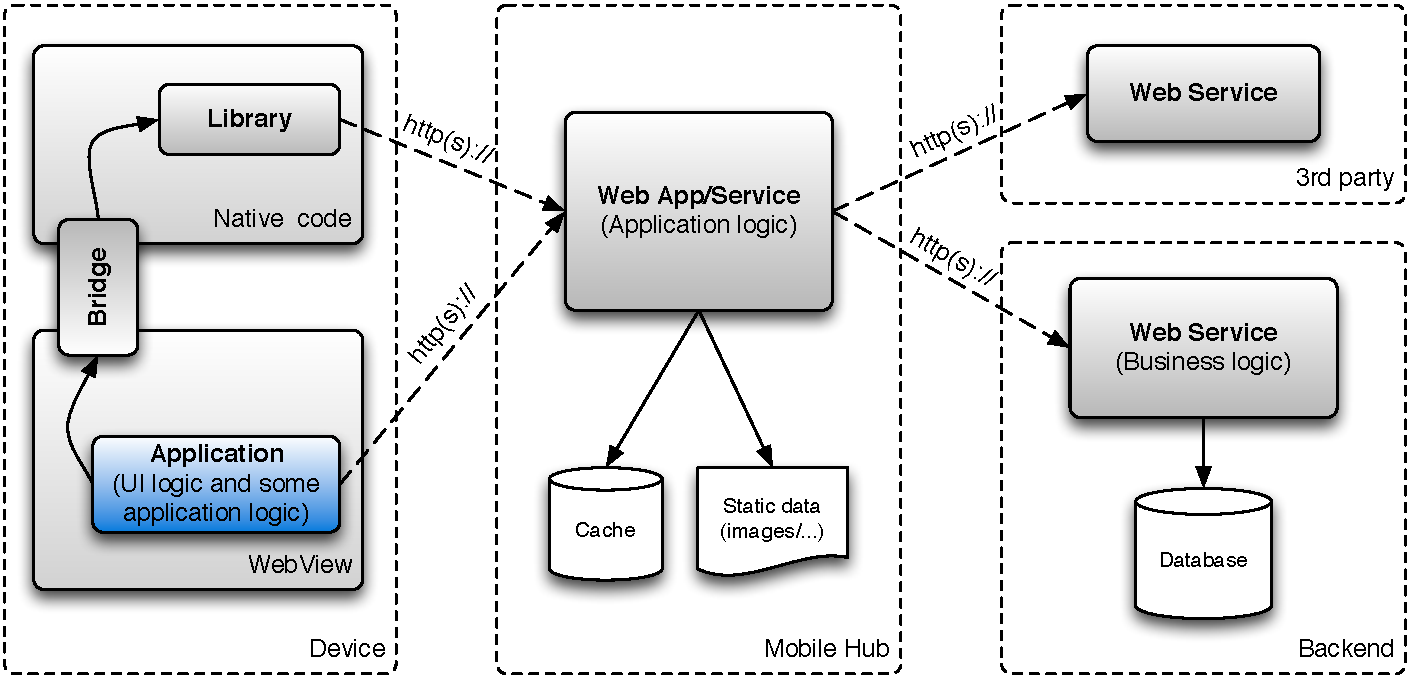
\includegraphics[width=\textwidth]{figs/hybrid.pdf}
        \caption{Architecture of a hybrid application. Based on \cite{Friese}}
        \label{fig:hybrid}
    \end{center}
\end{figure}

Because of the nature of the application, the performance is be similar to web applications. Unlike mobile web applications, hybrid applications are more flexible because they allow better integration with the device through the JavaScript bridge. This way, missing features can be implemented natively and accessed through said bridge. Another consequence of its nature is that hybrid applications do not use the native user interface elements and cannot provide the native look \& feel. 

The development cost of hybrid applications is similar to that of mobile web applications because wrapping web applications does not require any knowledge of the native SDK's. 

\subsection{Interpreted application}

Interpreted or runtime applications try to solve the platform differences by introducing an intermediary programming language. Instructions from that language are translated to native instructions at runtime. Interpreted applications are similar to Java applications on the desktop. From the outside, interpreted applications look just like native applications and can be distributed through online marketplaces. An interpreter or runtime is built right into the application, which increases the installation size of the application. This could be disadvantageous on low-end smartphones with limited storage capabilities. The architecture of an interpreted application is demonstrated in \fref{fig:interpreted}.

\begin{figure}[h]
    \begin{center}
        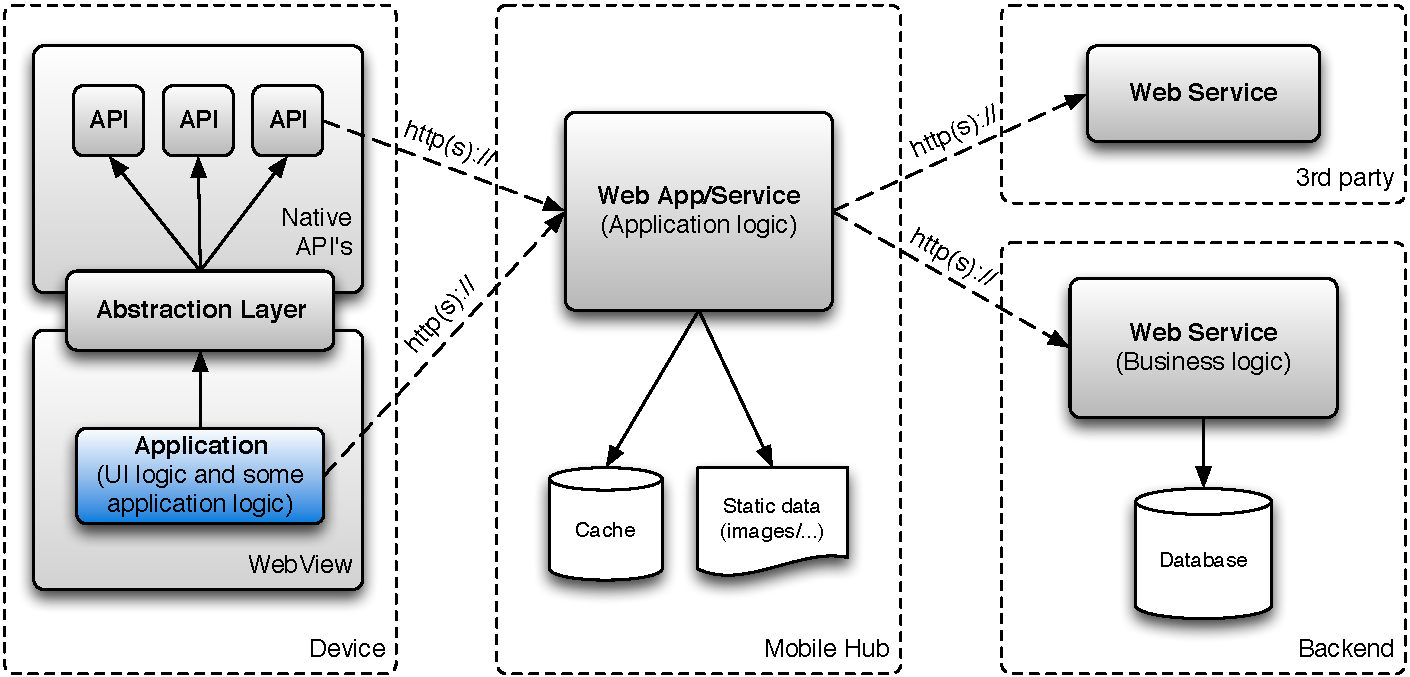
\includegraphics[width=\textwidth]{figs/interpreted.pdf}
        \caption{Architecture of an interpreted or runtime application. Based on \cite{Friese}}
        \label{fig:interpreted}
    \end{center}
\end{figure}

The performance of an interpreted application strongly depends on the interpreter itself and the interpreted programming language. In general, the performance is better than the performance of web applications but it is not as good as the performance of native applications. Because of the nature of interpreted applications, the native user interface elements can be used to provide a native look \& feel.

The development cost of interpreted applications is a higher than the cost of mobile web applications but lower than the cost of native applications. Developers need to be familiar with the SDK of the cross-platform tool but the application has to be developed only once and can be run on all supported platforms.

\subsection{Cross-compiled application}

In contrast to interpreted applications, instructions of cross-compiled are translated at compile time. The resulting application is not noticeably different from a native application because no runtime has to be included. This architecture is presented in \fref{fig:crosscompiled}. 

\begin{figure}[h]
    \begin{center}
        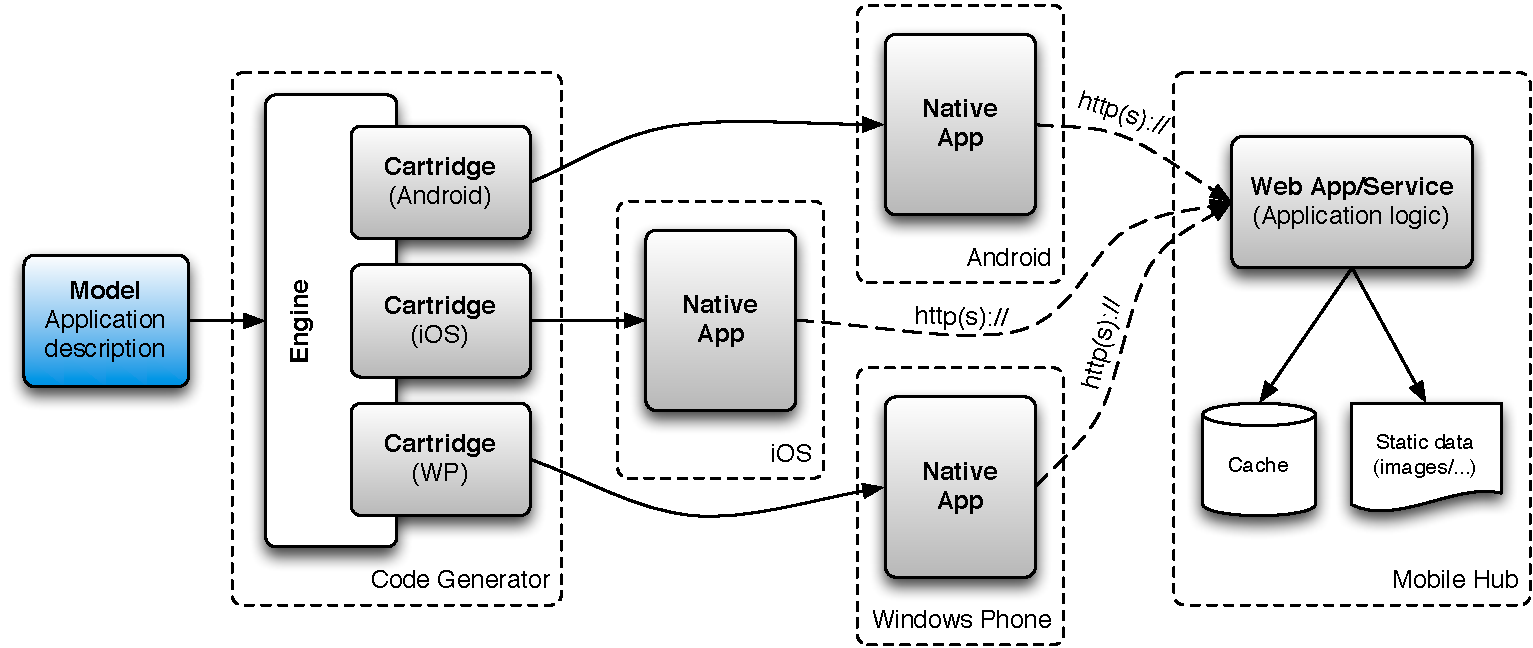
\includegraphics[width=\textwidth]{figs/crosscompiled.pdf}
        \caption{Architecture of a cross-compiled application. Based on \cite{Friese}}
        \label{fig:crosscompiled}
    \end{center}
\end{figure} 

Because the application only exists of machine code, the performance of cross-compiled applications is nearly identical to the performance of native applications. Cross-compiled applications can make use of the native user interface elements and consequently provide the native look \&feel. However, this sometimes requires custom bindings for each platform, increasing the amount of code that has to be written. 

The development costs of cross-compiled applications is similar to the costs of interpreted applications. Developers still need to be familiar with the SDK of the cross-platform tool but the application has to be developed only once and can be run on all supported platforms. Also, not all code can be reused in cross-compiled applications, which raises the development costs a little more.

\subsection*{Comparison of mobile architectures}

To conclude this section, the discussed architectures are compared side by side. The results are shown in \tref{tab:architectures}. Every architecture has both strengths and weaknesses. Therefore, the architecture must be chosen carefully, taking the client's wishes into account. 

\begin{table}[h]
    \begin{center}
        \begin{tabular}{lccccc}
            \hline
                            & Native      & Web         & Hybrid      & Interpreted & Cross-compiled\\
            \hline
            Performance     & high        & low         & low         & average     & high          \\
            Hardware access & \checkmark  & partial     & \checkmark  & \checkmark  & \checkmark    \\
            Look \& Feel    & native      & non-native  & non-native  & native      & native        \\
            Distribution    & store       & URL         & store       & store       & store         \\
            Cost            & high        & low         & low         & moderate    & moderate      \\
            \hline
        \end{tabular}
		\caption{
			Summary of cross platform mobile application development strategies.
		}
		\label{tab:architectures}
    \end{center}
\end{table}

\section{Software evaluation methodology}
\label{sec:sw-selection}

One of the goals of this thesis is to design a methodology for evaluating and selecting cross-platform tools. Based on their literature review \cite{Jadhav:2009}, \citet{Jadhav:2011} propose a generic software selection methodology. This methodology comprises of six steps:

\begin{enumerate}
    \item \textbf{Define selection criteria.} In the first stage, the selection criteria are defined. These are the functional and non-functional requirements that a software package has to meet.
    \item \textbf{Identify potential candidates.} During the second stage, a list of potential candidates is composed. During this search, any package that could be used to solve the targeted problem is considered a potential candidate. 
    \item \textbf{List selected alternatives.} In the third step, the selection criteria from the first stage are used to filter the list of potential candidates from the second stage: if a candidate does not satisfy the selection criteria, it is not considered for further evaluation.
    \item \textbf{Define evaluation criteria.} In the fourth stage, the evaluation criteria are defined. These are criteria that will be used to score a particular software package. These criteria should be arranged in a tree and every leaf node should be well-defined and measurable basic attribute.
    \item \textbf{Evaluate selected alternatives.} During the fifth phase, the software packages are evaluated. First, weights are assigned to the evaluation criteria from the fourth stage. Second, the software packages are rated with respect to the evaluation criteria. Third, an aggregated score is calculated for each software package.
    \item \textbf{Select the most suitable alternative.} In the final stage, all alternatives are ranked in order of decreasing aggregated score (which was calculated in the previous stage). The most suited software package will rank highest. However, selection is always human-dependable: additional cost-benefit analysis could be performed to identify the package with the best value, contract negotiations can influence the decision, etc. 
\end{enumerate}

In their first paper, \citet{Jadhav:2009} also suggest to include a validation stage to confirm that the selected package is indeed the most suited. 

\section{Multicriteria decision making (MCDM)}
\label{sec:mcdm}

The generic software selection methodology of \citet{Jadhav:2011} does not impose a particular technique for evaluating software packages. However, the last three stages of this methodology can be recognized as a multi-criteria decision making (MCDM) problem, for which a number of techniques are available. Multi-criteria decision making refers to making decisions in the presence of multiple --- often conflicting --- criteria. 

There are two types of MCDM problems: in multi-attribute decision making (MADM) problems, the decision maker tries to \emph{identify} the ``best'' alternative from a \emph{finite} set of alternatives with respect to multiple criteria or \emph{attributes}. In multi-objective decision making (MODM) problems, the decision maker tries to \emph{design} the ``best'' alternative from an \emph{infinite} set of possibilities with respect to multiple \emph{objectives} \cite{Kahraman:2008}. The software selection process clearly belongs to the category of MADM problems because the goal is to find the best alternative within a finite set of alternatives \cite{Jadhav:2009, Jadhav:2011}. 

There are numerous approaches to solve MADM problems. In the next subsections, a collection of approaches that are successfully applied in literature will be discussed. Every subsection will present a (high-level) description of the method and its strengths and weaknesses. Subsequently, every method is applied to a simple, running example.

The running example is as follows. Ethan has just graduated and has received three job offers. Every job is evaluated with respect to four criteria: the starting salary, distance to work (in km), degree of interest and career opportunities. Job 1 is an interesting position at a local start-up but it pays less. A large multinational offers job 2, which has a high reward and great career opportunities but is also further away from home. Job 3 is far away from home but combines great career opportunities with a good salary and interesting work. Note that the first two criteria are quantitative criteria, i.e. they can easily be mapped on a number. The last two criteria are qualitative criteria, i.e. they give a description but there is no straightforward mapping on a number. 

\subsection{Scoring models}

The first approach to solving MCDM problems is a collection of methods that have one thing in common: every alternative is assigned an arbitrary score with respect to one criterion and the scores for all criteria are aggregated into one final score. The final scores are then used to rank the alternatives.

Different methods are available to calculate the final score of a candidate \cite{Kahraman:2008}:

\begin{itemize}
    \item The ``dominance'' method can be used when one alternative  clearly outperforms the other alternatives with respect to at least one criterion and performs equally well with respect to the other criteria. 
    \item The ``maximin'' method calculates the total score of an alternative as the lowest score of all criteria scores of this alternative.
    \item The ``maximax'' method calculates the final score of an alternative as the highest score of all criteria scores of this alternative.
    \item With the ``conjunctive'' method, an alternative should exceed certain thresholds for \emph{all} criteria.
    \item With the ``disjunctive'' method, an alternative should exceed certain thresholds for \emph{at least one} criterion. 
    \item The ``additive weighting'' method calculates the total score of an alternative as the weighted \emph{sum} of the criteria scores and criteria weights.
    \item The ``weighted product'' method calculates the total score of an alternative as the weighted \emph{product} of the criteria scores and criteria weights.
\end{itemize}

The strength of these methods is that they are the easy to use. The weaknesses are that it (1) is hard to assign scores to qualitative criteria and definitely when there are many alternatives because humans can only deal with 7, plus or minus 2 pieces of information simultaneously and (2) different scales get mixed up \cite{Jadhav:2009, Miller:1956}. These weaknesses will become clear in the example.

\paragraph{Example}

Assume that Ethan has assigned weights to the four criteria in an arbitrary fashion and that he has also assigned scores to every alternative. Because this method requires a numerical value for each criterion, Ethan has created a value scale for ``interest'' and ``opportunities'': 0 represents satisfiable, 1 represents good and 2 represents excellent. Also, the distance property has been inverted such that a shorter distance is rewarded with a higher score. He has naively used the additive weighting method to aggregate the scores. The weights, scores, and resulting total scores are listed in \tref{tab:sm1}.

\begin{table}[h]
    \begin{center}
        \begin{tabular}{lrrrrr}
            \hline
            Alternative & Salary & Distance (km) & Interest & Opportunities & Total Score \\
            \hline
            Job 1       & 2000   & 1/5           & 2        & 0             & 400.62       \\
            Job 2       & 2800   & 1/30          & 0        & 2             & 560.80       \\
            Job 3       & 2600   & 1/60          & 1        & 1             & 520.70      \\
            \hline
            Weight      & 20\%   & 10\%          & 30\%     & 40\%          &             \\
            \hline
        \end{tabular}
        \caption{Naive demonstration of the additive weighting method.}
        \label{tab:sm1}
    \end{center}
\end{table}

From this first and naive attempt, Ethan would be inclined to choose the second job offer over the third one, and the third offer over the first one. However, there are a number of issues with this approach. The scores have different orders of magnitude, which affects the scaling. This can be solved by normalizing the scores, i.e. dividing each score by the sum of scores for a particular criterion. The new, normalized scores are listed in \tref{tab:sm2}.

\begin{table}[h]
    \begin{center}
        \begin{tabular}{lrrrrr}
            \hline
            Alternative & Salary & Distance (km) & Interest & Opportunities & Total Score \\
            \hline
            Job 1       & 0.27   & 0.80          & 0.67     & 0             & 0.33        \\
            Job 2       & 0.38   & 0.13          & 0        & 0.67          & 0.36        \\
            Job 3       & 0.35   & 0.07          & 0.33     & 0.33          & 0.31        \\
            \hline
            Weight      & 20\%   & 10\%          & 30\%     & 40\%          &             \\
            \hline
        \end{tabular}
        \caption{Improved version of the additive weighting method.}
        \label{tab:sm1}
    \end{center}
\end{table}

In the second attempt, the ranking of the alternatives has changed. This is caused by normalizing the scores before weighting. One problem remains unsolved though: the value scale for interest and opportunity criteria does not capture the distance between two successive values. The used scale is an ordinal scale, i.e. the elements of the scale have a well-defined order but the distance between elements is undefined. Scoring models are not suited to convert qualitative criteria into numbers.

\subsection{Analytic Hierarchy Process (AHP)}
\label{sec:ahp}

The second method is the Analytic Hierarchy Process (AHP) \cite{Saaty:1980}. This method, developed by Thomas L. Saaty, is widely used in multi-attribute decision making. The method can be used with both qualitative and quantitative criteria and calculates priorities (or weights) from pairwise comparison matrices by using the eigenvalue problem. 

The analytic hierarchy process consists of two stages. During the first stage, the factors that are important for the decision are organized into ``a hierarchic structure descending from an overall goal to criteria, subcriteria and alternatives in successive levels'' \cite{Saaty:1990}. Organizing the factors in such a structure helps the decision maker in getting an overview of the potentially complex relationships and also helps to assess the relative importance of the issues in each level. Structuring information in a tree is also backed by experiments of psychologist George Miller. He found that people can only deal with a few facts simultaneously; more precisely seven, plus or minus two \cite{Miller:1956}. 

During the second stage, both criteria and alternatives are compared in pairs. Every pairwise comparison results in a number that expresses the relation between two criteria or alternatives. \citet{Saaty:1990} proposes a fundamental scale (listed in \tref{tab:ahp-scale}) for expressing these relations. The results of the pairwise comparisons are combined in matrices and the analytic hierarchy process then establishes a ranking of the alternatives by calculating the principal right eigenvector of these comparison matrices. The next paragraphs will present an intuitive justification of the method.

\begin{table}
    \begin{center}
        \begin{tabular}{p{2.5cm}p{4cm}p{6cm}}
            \hline
            Intensity of importance on an absolute scale & Definition & Explanation \\
            \hline
            1 & Equal importance & Two activities contribute equally to the objective \\
            3 & Weak importance of one over another & Experience and judgement slightly favour one activity over another \\
            5 & Essential or strong importance & Experience and judgement strongly favour one activity over another \\
            7 & Very strong or demonstrated importance & An activity is favoured very strongly over another; its dominance is  demonstrated in practice \\
            9 & Absolute importance & The evidence favouring one activity over another is of the highest possible order of affirmation \\
            2, 4, 6, 8 & Intermediate values between adjacent scale values & When compromise is needed \\
            Reciprocals of above nonzero & \multicolumn{2}{p{10cm}}{If activity $i$ has one of the above nonzero numbers assigned with activity $j$, then $j$ has the reciprocal value when compared with $i$. This is a reasonable assumption.} \\
            Rationals & Ratios arising from the scale & If consistency were to be forced by obtaining $n$ numerical values to span the matrix \\
            \hline
        \end{tabular}
        \caption{The fundamental scale for pairwise comparison\cite{Saaty:1990}}
        \label{tab:ahp-scale}
    \end{center}
\end{table}

Consider $n$ alternatives $A_1, A_2, \ldots, A_n$ and a quantitative criterion $X$, i.e. $X$ can be expressed with an exact number. The value of a certain alternative $A_i$ with respect to criterion $X$ is given by $w_i$. For instance, $A_i$ could be $n$ stones and $X$ could be their weight, measured in grams. The ratios between any two alternatives (with respect to property $X$) can now be summarized in a matrix
\begin{gather*}
    A = %
    \begin{bmatrix}
        w_1/w_1 & w_1/w_2 & \ldots & w_1/w_n \\
        w_2/w_1 & w_2/w_2 & \ldots & w_2/w_n \\
        \vdots  & \vdots  &        & \vdots  \\
        w_n/w_1 & w_n/w_2 & \ldots & w_n/w_n    
    \end{bmatrix}.
\end{gather*}

Note that (1) $A$ is reciprocal, i.e. $a_{ij} = 1 / a_{ji}$ and (2) the elements on the diagonal are ones. This is easy to understand because there cannot be any difference between two identical objects.

If any row of $A$ were to be multiplied by a vector $\vec{w} = (w_1, w_2, \ldots, w_n)^T$, the multiplication would yield a row of identical entries $w_i, w_i, \ldots, w_i$. This is only true in the case of perfect information. In most multi-criteria decision making problems, information is incomplete, incorrect or it simply cannot be represented by numbers (because the criterion describes a qualitative property) and the exact ratios cannot be calculated. In that case, the ratios $a_{ij} = w_i/w_j$ can be estimated by an expert, who is allowed to make (small) errors in judgement. These estimates $a'_{ij}$ make up a new matrix $A'$. Then, the result of the aforementioned multiplication is a row of statistically scattered values around the actual value $w_i$. Therefore, it seems reasonable to represent $w_i$ by the average of these values:
\begin{gather*}
    w'_i = \frac{1}{n} \sum_{j=1}^{n} a'_{ij} w'_j \quad i = 1, 2, \ldots, n
\end{gather*}

This resulting system can be solved for $\vec{w'} = (w'_1, w'_2, \ldots, w'_n)^T$ if $n$ is allowed to change. The problem then reads:
\begin{gather*}
    w'_i = \frac{1}{\lambda_{max}} \sum_{j=1}^{n} a'_{ij} w'_j \quad i = 1, 2, \ldots, n
\end{gather*}
which is equivalent to the eigenvalue problem $A' \vec{w'} = \lambda_{max} \vec{w'}$. The eigenvector $\vec{w'}$, which is unique up to within a multiplicative constant, has to be normalized by dividing its entries by their sum to obtain a \emph{priority vector}, i.e. a vector of appropriate weights or scores for the considered alternatives. 

The eigenvalue problem has a number of interesting properties. Reconsider $A$. This is a positive, reciprocal matrix and it is also consistent, i.e. all entries satisfy the condition
\begin{gather*}
    a_{jk} = \frac{a_{ik}}{a_{ij}} = \frac{w_i}{w_k} \times \frac{w_j}{w_i} \quad i, j, k = 1, \ldots, n.
\end{gather*}
In other words, the alternatives form a chain which also represents their ranking. Because of this property, all rows of $A$ are linearly dependent and consequently, $A$ has rank one. This also implies that all eigenvalues are zero, except one. In every matrix, the sum of eigenvalues is equal to the sum of elements on the diagonal (also known as the trace of a matrix). Hence, $tr(A) = n$, the order of $A$.

In the presence of small inconsistencies (where $A$ is approximated by $A'$), $\vec{w'}$ is a good estimate of $\vec{w}$ as long as $A'$ is reciprocal because it can be shown that small perturbations of $a_{ij}$ do not lead to large perturbations of $\lambda_{max}$ and $\vec{w'}$ \cite{Saaty:1980}. However, the amount of inconsistency should be measurable in order to decide whether it is small or not. It turns out that the amount of inconsistency is proportional to the difference between the expected eigenvalue $n$ and the actual eigenvalue $\lambda_{max}$.

\citet{Saaty:1980} defines a number, called the \emph{consistency index}, $CI = (\lambda_{max} - n) / (n - 1)$, which measures the amount of inconsistency in a given judgement matrix. This consistency index is then compared to the average consistency index of a large number of random reciprocal matrices of the same order, called the \emph{random index} (RI). These random indices can be found in \tref{tab:ri}. If the \emph{consistency ratio} $CR = CI / RI$ is $0.1$ or less, the estimate $\vec{w'}$ is accepted. Otherwise, new judgements should be collected in order to improve consistency.

\begin{table}
    \begin{center}
        \begin{tabular}{l*{9}{|c}}
            n & 1 & 2 & 3 & 4 & 5 & 6 & 7 & 8 & 9\\
            \hline
            RI & 0 & 0 & 0.58 & 0.90 & 1.12 & 1.24 & 1.32 & 1.41 & 1.45
        \end{tabular}
        \caption{Random indices (RI) for reciprocal matrices of order 1 to 9}
        \label{tab:ri}
    \end{center}
\end{table}

The strengths of the AHP are that it (1) enables decision makers to structure a problem into a hierarchy, (2) provides a powerful approach for handling both quantitative and qualitative criteria and (3) can deal with inconsistencies. The weaknesses of AHP are that it (1) is a time-consuming method due to the large number of pairwise comparisons and (2) is susceptible to rank-reversal, i.e. the ranking may change when new alternatives are added \cite{Jadhav:2009}.

\paragraph{Example}

In this example, Ethan uses the AHP method to assist him in choosing a job offer. The goal, which is the root node of the hierarchy, is obviously to select a job offer. The four criteria (salary, distance to work, interest and career opportunities) are children of the root node and the alternatives are children of the criterion nodes. \fref{fig:ahp-hierarchy} illustrates the hierarchy.

\begin{figure}
    \begin{center}
        \begin{pspicture}(0, 0)(12, 4)
            \psnode(6, 4){G}{Goal}
            \psnode(2.4, 2){C1}{Salary}
            \psnode(4.8, 2){C2}{Distance}
            \psnode(7.2, 2){C3}{Interest}
            \psnode(9.6, 2){C4}{Opportunities}
            \psnode(3, 0){O1}{Offer 1}
            \psnode(6, 0){O2}{Offer 2}
            \psnode(9, 0){O3}{Offer 3}
            
            \ncline[nodesep=3pt]{G}{C1}
            \ncline[nodesep=3pt]{G}{C2}
            \ncline[nodesep=3pt]{G}{C3}
            \ncline[nodesep=3pt]{G}{C4}
            
            \ncline[nodesep=3pt]{O1}{C1}
            \ncline[nodesep=3pt]{O1}{C2}
            \ncline[nodesep=3pt]{O1}{C3}
            \ncline[nodesep=3pt]{O1}{C4}
            
            \ncline[nodesep=3pt]{O2}{C1}
            \ncline[nodesep=3pt]{O2}{C2}
            \ncline[nodesep=3pt]{O2}{C3}
            \ncline[nodesep=3pt]{O2}{C4}
            
            \ncline[nodesep=3pt]{O3}{C1}
            \ncline[nodesep=3pt]{O3}{C2}
            \ncline[nodesep=3pt]{O3}{C3}
            \ncline[nodesep=3pt]{O3}{C4}
        \end{pspicture}
        \caption{The decision hierarchy of the running example.}
        \label{fig:ahp-hierarchy}
    \end{center}    
\end{figure}

First, Ethan has to decide upon the relative importance of every combination of two criteria. The comparison matrix is a 4-by-4 matrix but the diagonal carries only ones and only half of the remaining judgements is needed because the matrix must be reciprocal. Hence, 6 pairwise comparisons have to be made. Ethan uses Saaty's fundamental scale (see \tref{tab:ahp-scale}) to rate the criteria. For instance, Ethan is convinced that the salary is more important than the distance, which is illustrated in \tref{tab:ahp-criteria} together with the other scores. The consistency ratio is less than 0.1

\begin{table}[h]
    \begin{center}
        \begin{tabular}{lccccr}
            \hline
                          & Salary          & Distance & Interest        & Opportunities   & Priority vector \\
            \hline
            Salary        & $1$             & $5$      & $\lsfrac{1}{3}$ & $\lsfrac{1}{3}$ & $0.1525$        \\
            Distance      & $\lsfrac{1}{5}$ & $1$      & $\lsfrac{1}{7}$ & $\lsfrac{1}{7}$ & $0.0450$        \\
            Interest      & $3$             & $7$      & $1$             & $\lsfrac{1}{3}$ & $0.2919$        \\        
            Opportunities & $3$             & $7$      & $3$             & $1$             & $0.5106$        \\    
            \hline
            \multicolumn{6}{r}{$\lambda_{max} = 4.2281$, $CI = 0.0760$, $CR=0.08$}                           \\
            \hline
        \end{tabular}
        \caption{Comparison of criteria}
        \label{tab:ahp-criteria}
    \end{center}
\end{table}

Second, Ethan has to score the alternatives in a similar fashion with respect to the criteria. The first two criteria are quantitative criteria and these numbers are used to form the ratios. In this case, the comparison matrix is both reciprocal and consistent. Consequently, the consistency ratio is zero. The last two criteria are qualitative criteria and are scored using Saaty's scale. The judgements and resulting priority vectors are listed in \tref{tab:ahp-alternatives}.


\begin{table}[h]
    \begin{tabular}{lcccr}
        \hline
        \textbf{Salary} & J1                    & J2                    & J3                    & Priority \\
        \hline
        J1              & $1$                   & $\lsfrac{2000}{2800}$ & $\lsfrac{2000}{2600}$ & $0.2703$ \\
        J2              & $\lsfrac{2800}{2000}$ & $1$                   & $\lsfrac{2800}{2600}$ & $0.3784$ \\
        J3              & $\lsfrac{2600}{2000}$ & $\lsfrac{2600}{2800}$ & $1$                   & $0.3513$ \\        
        \hline
        \multicolumn{5}{r}{$\lambda_{max} = 3$, $CI = 0$}                                                  \\
        \hline
    \end{tabular}
    \hfill
    \begin{tabular}{lcccr}
        \hline
        \textbf{Distance} & J1               & J2                & J3                & Priority \\
        \hline
        J1                & $1$              & $\lsfrac{30}{5}$  & $\lsfrac{60}{5}$  & $0.8000$ \\
        J2                & $\lsfrac{5}{30}$ & $1$               & $\lsfrac{60}{30}$ & $0.1333$ \\
        J3                & $\lsfrac{5}{60}$ & $\lsfrac{30}{60}$ & $1$               & $0.0667$ \\        
        \hline
        \multicolumn{5}{r}{$\lambda_{max} = 3$, $CI = 0$}                                       \\
        \hline
    \end{tabular}
    \\\vspace{1em}\\
    \begin{tabular}{lcccr}
        \hline
        \textbf{Interest} & J1              & J2    & J3              & Priority    \\
        \hline
        J1                & $1$             & $7$   & $3$             & $0.6694$    \\
        J2                & $\lsfrac{1}{7}$ & $1$   & $\lsfrac{1}{3}$ & $0.0880$    \\
        J3                & $\lsfrac{1}{3}$ & $3$   & $1$             & $0.2426$    \\        
        \hline
        \multicolumn{5}{r}{$\lambda_{max} = 3.0070$, $CI = 0.0035$, $CR = 0.006$}   \\
        \hline
    \end{tabular}
    \hfill
    \begin{tabular}{lcccr}
        \hline
        \textbf{Opportunities} & J1  & J2              & J3              & Priority \\
        \hline
        J1                     & $1$ & $\lsfrac{1}{7}$ & $\lsfrac{1}{5}$ & $0.0668$ \\
        J2                     & $7$ & $1$             & $5$             & $0.7147$ \\
        J3                     & $5$ & $\lsfrac{1}{5}$ & $1$             & $0.2185$ \\        
        \hline
        \multicolumn{5}{r}{$\lambda_{max} = 3.1827$, $CI = 0.0914$, $CR = 0.16$}    \\
        \hline
    \end{tabular}
    \caption{Comparison of job offers with respect to the four criteria}
    \label{tab:ahp-alternatives}
\end{table}

Finally, all scores are combined into a total score $a_i$ by calculating
\begin{gather*}
    a_i = \sum_{i = 1}^{4} c_i w_i
\end{gather*}
where $c_i$ is the priority of a particular criterion and $w_i$ is the priority of the alternative with respect to this criterion. The vector of total scores is then $(0.3067, 0.4543, 0.2389)^T$.

\subsection{Fuzzy MCDM}
\label{sec:fuzzy}

In 1965, \citet{Zadeh:1965} introduced the concept of fuzzy sets. Five years later, \citet{Bellman:1970} applied this concept to multi-criteria decision making problems, which allows decision makers to express constraints like ``the cost of $A$ should be substantially lower than $\alpha$''.

The approach is based on the observation that ``most real world decision making processes take place in an environment in which the goals, the constraints and consequences of possible actions are not known precisely'' \cite{Bellman:1970}. Usually, this imprecision is associated with randomness, which is fundamentally different from fuzziness. Fuzziness is a type of imprecision that is associated with fuzzy sets. ``A fuzzy set is a class of objects in which there is no sharp boundary between those objects that belong to the class and those that do not'' \cite{Bellman:1970}. The set of blue objects is an example of a fuzzy set. More formally, if $X = \left\{x\right\}$ denotes a set of alternatives, then the fuzzy set $A$ in $X$
\begin{gather*}
    A = \left\{\left(x, \mu_A\left(x\right)\right)\right\}, \quad x \in X
\end{gather*}
is a set of ordered pairs where $\mu_A\left(x\right)$ is called the membership degree of $x$ in $A$. $\mu_A : X \rightarrow M$ is a function from a space $X$ to a membership space $M$ where $M = [0, 1]$ \cite{Bellman:1970}.

A decision process is typically comprised of three ingredients: a set of alternatives, a set of constraints and a performance function that indicates the gain (or loss) associated with each alternative. In a fuzzy environment, the goals and/or constraints make up classes of alternatives that do not have crisp boundaries. A fuzzy decision is then an intersection of the given goals and constraints. More formally, if $X = \left\{x\right\}$ is a given set of alternatives, then a (fuzzy) goal $G$ is given by a fuzzy set $G$ in $X$. The membership function $\mu_G\left(x\right)$ indicates to which degree a particular alternative $x$ satisfies the goal $G$. Such a function Similarly, a (fuzzy) constraint $C$ is given by a fuzzy set $C$ in $X$ and the degree to which a certain alternative $x$ satisfies the constraint $C$ is given by $\mu_C\left(x\right)$.

The decision is then an intersection of the goal and the constraint:
\begin{gather*}
    D = G \cap C
\end{gather*}
where $D$ is a fuzzy set, resulting from the intersection of $G$ and $C$. Correspondingly, the membership function $\mu_D\left(x\right) = \mu_G\left(x\right) \wedge \mu_C\left(x\right)$ is a function of the membership functions of $G$ and $C$. In case of intersection, $\mu_D\left(x\right) = min\left(\mu_G\left(x\right), \mu_C\left(x\right)\right)$.
 
More generally, a multi-criteria decision making problem can have $n$ goals $G_1, \ldots, G_n$ and $m$ constraints $C_1, \ldots, C_m$ and the resulting decision is the intersection of goals and constraints:
\begin{gather*}
    D = G_1 \cap \ldots G_n \cap C_1 \cap \ldots \cap C_n
\end{gather*}
In fact, other interpretations of ``intersection'' can be used as well. The decision is then called a ``confluence'' of goals and constraints.

The strengths of the fuzzy MCDM approach are that (1) linguistic terms can be used for evaluation and (2) improves decision making in the presence of vagueness and ambiguity. The weakness of the approach is that it does not specified how the membership functions should be defined.

\paragraph{Example} The running example has one goal and four criteria. These can be translated into four goals (great salary, nice driving distance, great job content, great career opportunities) and four constraints (affordable salary, satisfiable distance to work, satisfiable job content, satisfiable job opportunities). That is, every criterion defines both a goal and a constraint. Next, the membership functions should be defined. However, it is not specified how to define these functions. For the sake of simplicity, this example this example will only discuss two membership functions of one criterion. Assume that Ethan thinks that the tipping point for an affordable salary is 1900 euro. The membership function could then be defined as:
\begin{gather*}
    \mu_{\text{Affordable Salary}}\left(x\right) = \frac{1}{1 + 1.05^{1900 - x}}
\end{gather*}
Similarly, the tipping point for a great salary is 2800 euro but is also spread out over a larger range:
\begin{gather*}
    \mu_{\text{Great Salary}}\left(x\right) = \frac{1}{1 + 1.005^{2800 - x}}
\end{gather*}
Both functions are visualized in \fref{fig:fuzzy}. The membership degree of the decision can now be calculated as the minimum of these two functions:
\begin{align*}
    \mu_{D}\left(2000\right) & = 0.00035 \\
    \mu_{D}\left(2800\right) & = 0.5     \\
    \mu_{D}\left(2600\right) & = 0.12025 
\end{align*}

\begin{figure}[h]
    \begin{center}
        \psset{lly=-0.5cm}
        \begin{psgraph}[Dx=100, Dy=0.2, Ox=1800](1800,0)(3000,1){10cm}{5cm}
            \psplot[linecolor=blue,linewidth=1pt,algebraic=true,plotpoints=2000]{1800}{3000}{1/(1+1.05^(1900 - x))}
            \psplot[linecolor=red,linewidth=1pt,algebraic=true,plotpoints=2000]{1800}{3000}{1/(1+1.01^(2800 - x))}
        \end{psgraph}
        \caption{Visualization of $\mu_{\text{Affordable Salary}}$ (blue) and $\mu_{\text{Great Salary}}$ (red)}
        \label{fig:fuzzy}
    \end{center}
\end{figure}

 
 













